\documentclass[10pt,twocolumn]{article}

\usepackage[margin=0.70in,columnsep=0.24in]{geometry}
\usepackage[T1]{fontenc}
\usepackage[utf8]{inputenc}
\usepackage{lmodern}
\usepackage{microtype}
\usepackage{amsmath,amssymb,amsthm,bm,mathtools}
\usepackage{booktabs,multirow,array}
\usepackage{graphicx}
\usepackage{xcolor}
\usepackage{algorithm}
\usepackage[noend]{algpseudocode}
\usepackage{caption}
\usepackage{subcaption}
\usepackage{siunitx}
\usepackage[numbers,sort&compress]{natbib}
\usepackage{hyperref}
\usepackage[capitalize,noabbrev]{cleveref}

\hypersetup{
  pdftitle={Discriminative Energy Component Analysis},
  pdfauthor={Rongzhou (Lachlan) Chen},
  colorlinks=true,
  citecolor=blue!55!black,
  linkcolor=blue!55!black,
  urlcolor=blue!55!black
}
\graphicspath{
  {../../experiments/run1/results/theory/}
  {../../experiments/run1/results/quantum/}
  {../../experiments/run1/results/classical/}
}
\sisetup{detect-all}

\newtheorem{theorem}{Theorem}
\newtheorem{proposition}[theorem]{Proposition}
\newtheorem{corollary}[theorem]{Corollary}
\newtheorem{lemma}[theorem]{Lemma}
\theoremstyle{definition}
\newtheorem{definition}[theorem]{Definition}
\theoremstyle{remark}
\newtheorem{remark}[theorem]{Remark}

\newcommand{\Tr}{\operatorname{Tr}}
\newcommand{\diag}{\operatorname{diag}}
\newcommand{\offdiag}{\operatorname{offdiag}}
\newcommand{\argmax}{\operatorname*{arg\,max}}
\newcommand{\E}{\mathbb{E}}
\newcommand{\C}{\mathbb{C}}
\newcommand{\R}{\mathbb{R}}
\newcommand{\calA}{\mathcal{A}}
\newcommand{\calE}{\mathcal{E}}
\newcommand{\rhohat}{\widehat{\rho}}

\title{\textbf{Discriminative Energy Component Analysis:}\\
Optimal Commuting Measurements and Spectral Quadratic Classification}
\author{Rongzhou (Lachlan) Chen\\
\small Independent Research Draft\\
\small \texttt{https://github.com/lachlanchen/discriminative-energy-component-analysis}}
\date{July 2026}

\begin{document}
\maketitle

\begin{abstract}
Principal component analysis orders directions by total variance, not by
class discrimination.  Eigen-Component Analysis (ECA) instead squares
orthogonal projections and assigns the resulting directional energies to
classes, but its precise optimization target, quantum interpretation, and
limits have remained unclear.  We reformulate this idea as
\emph{Discriminative Energy Component Analysis} (DECA): minimum-error state
discrimination under a shared-eigenbasis, or commuting-measurement,
constraint.  A common unitary is provably redundant for an unrestricted
positive operator-valued measure (POVM), so its only operational role is
measurement compression.  Under this constraint, we prove that the optimal
fixed-basis decoder is hard; binary DECA has a closed-form eigensolution equal
to the known Helstrom optimum; commuting multiclass ensembles are exact; and
the loss relative to the optimal POVM is bounded by a joint-diagonalization
residual.  For noncommuting multiclass problems we give a monotone Jacobi
algorithm with analytical two-dimensional updates.  We also separate
single-shot PVM-DECA from Spectral-DECA, which retains the magnitude of each
class-difference eigenvalue for deterministic quadratic classification.
Qiskit Aer simulations verify ancilla-free PVM and Naimark-dilated POVM
circuits to maximum total-variation error $0.0073$.  In 1,100 repeated
cross-validation fits on ten datasets, DECA validates the intended
second-order mechanism but does not generally outperform classical
baselines.  These results establish a rigorous resource--accuracy boundary,
not a quantum-speedup or universal-accuracy claim.
\end{abstract}

\section{Introduction}
\label{sec:introduction}

Variance and discrimination are different objectives.  Principal component
analysis (PCA) chooses directions that explain total second-moment energy,
including nuisance variation shared by all classes.  A classifier instead
needs directions whose responses differ across classes.  Fisher's linear
discriminant analysis (LDA) addresses this distinction through class means
\cite{fisher1936}; quadratic discriminant analysis (QDA), common spatial
patterns, and common principal components expose complementary second-order
structure \cite{friedman1989,flury1984,ramoser2000}.  The motivating question
of this work is narrower:
\begin{quote}
Can a single orthogonal basis be ordered and allocated by
\emph{class-conditional energy contrast}, rather than total variance, while
remaining analytically tractable and physically measurable?
\end{quote}

The original ECA preprint \cite{chen2020preprint} and the later ISCAS paper
\cite{chen2025eca} proposed squared orthogonal components,
\begin{equation}
  z_j(x)=|p_j^\dagger \phi(x)|^2,
  \label{eq:energy_feature}
\end{equation}
followed by class weights.  This construction is linear in $z(x)$ but is a
structured quadratic classifier in the encoded input $\phi(x)$.  When the
weights are nonnegative and sum to one across classes for every component,
the class operators are a commuting POVM.  This observation is the starting
point here.

Quantum state discrimination already supplies the binary Helstrom
measurement \cite{helstrom1976}, general POVM optimization by semidefinite
programming (SDP) \cite{eldar2003}, and the square-root or Pretty Good
Measurement (PGM) \cite{hausladen1994}.  These tools have also been applied to
classical supervised classification
\cite{sergioli2019,giuntini2021,lloyd2020,cruzeiro2023,hwang2024}.
Consequently, ``using a density matrix'' or ``using Helstrom'' is not a
novelty claim.  The unresolved issue is what remains of ECA after those known
facts are imposed exactly.

\paragraph{Contributions.}
This paper makes four scoped contributions.
\begin{enumerate}
  \item We identify ECA with a commuting-measurement constraint and prove that
  a shared unitary is irrelevant to an unrestricted POVM but meaningful as a
  compression of measurement resources.
  \item We analytically eliminate the soft component-to-class decoder,
  derive binary and commuting-multiclass exactness, prove a computable
  off-diagonal residual bound, and expose the unavoidable $K>d$ output
  limitation of a $d$-dimensional PVM.
  \item We introduce a monotone multiclass Jacobi-DECA procedure and separate
  the single-shot PVM rule from a spectral observable rule that preserves the
  magnitudes of discriminative eigenvalues.
  \item We provide tested classical, SDP, and Qiskit implementations; validate
  all stated identities numerically; and report both positive and negative
  results over controlled ensembles and public datasets.
\end{enumerate}

We do \emph{not} claim quantum speedup, privacy, hardware power or latency
advantages, or universal predictive superiority.

\section{Related Work and Positioning}
\label{sec:related}

\subsection{Discriminative second-order representations}

LDA finds a mean-separating subspace relative to within-class scatter
\cite{fisher1936}.  QDA assigns each class an unrestricted covariance model,
while regularized discriminant analysis interpolates between linear and
quadratic rules \cite{friedman1989}.  Common spatial patterns diagonalize two
covariance matrices to contrast class-specific variance and are widely used
for EEG decoding \cite{ramoser2000}.  Flury's common principal component
model assumes several covariance matrices share eigenvectors
\cite{flury1984}.  Approximate joint diagonalization and Jacobi plane
rotations provide computational tools when exact commutation fails
\cite{bunsegerstner1993,cardoso1996}.

DECA is closest to these methods statistically: its sufficient statistics are
class-conditional means of rank-one energy operators.  It differs from
unrestricted QDA by forcing class quadratic forms to share a basis, and from
PCA by ordering directions through class contrast rather than pooled
variance.  The shared-basis assumption is a bias that can either reduce
estimation variance or cause severe underfitting.

\subsection{Quantum state discrimination classifiers}

For a known binary ensemble, the Helstrom measurement minimizes single-copy
Bayes error \cite{helstrom1976}.  Multiclass minimum-error discrimination is a
convex SDP \cite{eldar2003}; PGM is a closed-form feasible alternative
\cite{hausladen1994}.  Sergioli \emph{et al.} constructed class density
patterns and a Helstrom quantum centroid classifier \cite{sergioli2019}.
Giuntini \emph{et al.} extended state-discrimination ideas to supervised
multiclass classification \cite{giuntini2021}.  Lloyd \emph{et al.} studied
trainable embeddings whose trace distance is paired with a Helstrom
measurement \cite{lloyd2020}.  Later work developed PGM and SDP
classifiers \cite{cruzeiro2023} and efficient simulations of multicopy
Helstrom rules \cite{hwang2024}.

Our binary solution is an independent reduction of the ECA objective to the
known Helstrom result, not a new state-discrimination theorem.  The original
content lies in the constrained-measurement formulation, hard-decoder
elimination, multiclass residual analysis, Jacobi objective, spectral/PVM
distinction, and end-to-end resource study.

\section{Problem Formulation}
\label{sec:problem}

Let an input be encoded as a unit vector
$\phi(x)\in\C^d$, with pure-state operator
\begin{equation}
  \rho_x=\phi(x)\phi(x)^\dagger,\qquad \Tr(\rho_x)=1.
\end{equation}
For class $c\in\{1,\ldots,K\}$, define
\begin{equation}
  \rho_c=\E[\rho_x\mid y=c],\qquad A_c=\pi_c\rho_c,
  \label{eq:class_operators}
\end{equation}
where $\pi_c$ is the class prior.  Thus $A_c\succeq0$ and
$\sum_c\Tr(A_c)=1$.

The general minimum-error measurement is
\begin{equation}
  S_{\mathrm{POVM}}^\star
  =
  \max_{\substack{E_c\succeq0\\\sum_cE_c=I}}
  \sum_{c=1}^K \Tr(A_cE_c).
  \label{eq:povm_primal}
\end{equation}
Its dual is
\begin{equation}
  S_{\mathrm{POVM}}^\star
  =
  \min_Y \Tr(Y)
  \quad\text{s.t.}\quad Y\succeq A_c\quad\forall c.
  \label{eq:povm_dual}
\end{equation}
We use \cref{eq:povm_primal} as a numerical oracle, not as a contribution.

\begin{proposition}[Shared-unitary redundancy]
\label{prop:unitary_redundancy}
For every unitary $U$,
\[
S_{\mathrm{POVM}}^\star(\{UA_cU^\dagger\})
=S_{\mathrm{POVM}}^\star(\{A_c\}).
\]
\end{proposition}
\begin{proof}
The map $E_c\mapsto UE_cU^\dagger$ is a bijection on feasible POVMs and
preserves every trace term by cyclicity.
\end{proof}

\Cref{prop:unitary_redundancy} prevents a common conceptual error: a learned
unitary cannot create information if the subsequent measurement is
unrestricted.  It matters only when the measurement family, circuit depth, or
number of outcomes is restricted.

\section{DECA as an Optimal Commuting Measurement}
\label{sec:theory}

Restrict all effects to a shared unitary basis
$P=[p_1,\ldots,p_d]$:
\begin{equation}
  E_c=P\diag(\ell_{1c},\ldots,\ell_{dc})P^\dagger,
  \quad
  \ell_{jc}\ge0,\quad\sum_c\ell_{jc}=1.
  \label{eq:commuting_effect}
\end{equation}
Let $a_{jc}(P)=p_j^\dagger A_cp_j$.  The success is
\begin{equation}
  S(P,L)=\sum_{j,c}\ell_{jc}a_{jc}(P).
\end{equation}

\begin{theorem}[Hard-decoder optimality]
\label{thm:hard_decoder}
For fixed $P$, an optimal decoder exists at a vertex of every row simplex:
\begin{align}
  \ell_{jc}^\star
  &=\bm{1}\!\left[c=\argmax_r a_{jr}(P)\right],
  \nonumber\\
  S_{\mathrm{DECA}}(P)
  &=\sum_j\max_c a_{jc}(P).
  \label{eq:deca_objective}
\end{align}
\end{theorem}
\begin{proof}
Each row $\ell_{j:}$ appears in an independent linear program over the
probability simplex.  A maximizing vertex assigns all mass to a largest
coefficient.
\end{proof}

Thus soft weights are unnecessary for the minimum-error objective.  The
optimal commuting POVM can be chosen as a projective measurement followed by
a classical outcome-to-class map.

\subsection{Binary closed form}

Let $\Delta=A_1-A_2$.  For every $P$,
\begin{equation}
S_{\mathrm{DECA}}(P)
=\frac12\left[
1+\left\|\diag(P^\dagger\Delta P)\right\|_1
\right].
\label{eq:binary_basis_objective}
\end{equation}

\begin{theorem}[Binary DECA equals Helstrom]
\label{thm:binary}
If $P$ is an eigenbasis of $\Delta$, then
\begin{equation}
  S_{\mathrm{DECA}}^\star
  =\frac12(1+\|\Delta\|_1)
  =S_{\mathrm{POVM}}^\star.
  \label{eq:helstrom}
\end{equation}
Outcome $j$ is assigned according to the sign of
$\lambda_j(\Delta)$.
\end{theorem}
\begin{proof}
By the Schur--Horn theorem,
$\diag(P^\dagger\Delta P)\prec\lambda(\Delta)$
\cite{bhatia1997}.  The $\ell_1$ norm is convex and symmetric, hence
$\|\diag(P^\dagger\Delta P)\|_1\le\|\lambda(\Delta)\|_1$.
An eigenbasis attains equality.  Substitution into
\cref{eq:binary_basis_objective} yields the known Helstrom formula.
\end{proof}

The magnitude $|\lambda_j|$ is the contribution of component $j$ to total
trace-distance discrimination.  This gives a principled low-rank ordering:
retain the smallest $r$ satisfying
$\sum_{j\le r}|\lambda|_{(j)}/\sum_j|\lambda_j|\ge\eta$.

\subsection{Multiclass exactness and approximation}

\begin{theorem}[Commuting multiclass exactness]
\label{thm:commuting}
If $[A_c,A_r]=0$ for all $c,r$, then a common eigenbasis $P$ satisfies
$S_{\mathrm{DECA}}(P)=S_{\mathrm{POVM}}^\star$.
\end{theorem}
\begin{proof}
In the common eigenbasis, only the diagonal entries of any feasible POVM
contribute to \cref{eq:povm_primal}.  Those entries form a stochastic decoder,
whose optimum is the hard decoder in \cref{thm:hard_decoder}.
\end{proof}

For a general basis define
\begin{equation}
  P^\dagger A_cP=D_c+O_c,\quad
  D_c=\diag(P^\dagger A_cP),
\end{equation}
and
\begin{equation}
  R_{\mathrm{off}}(P)
  =
  \left(\sum_c\|O_c\|_F^2\right)^{1/2}.
  \label{eq:residual}
\end{equation}

\begin{theorem}[POVM gap bound]
\label{thm:gap}
For every unitary $P$,
\begin{equation}
0\le
S_{\mathrm{POVM}}^\star-S_{\mathrm{DECA}}(P)
\le \sqrt{d}\,R_{\mathrm{off}}(P).
\label{eq:gap_bound}
\end{equation}
\end{theorem}
\begin{proof}
Write an optimal POVM in the $P$ basis as $\{F_c\}$.  Its diagonal part is a
feasible soft decoder, no better than the fixed-basis hard optimum.  The
remaining contribution is at most
$\sum_c|\Tr(F_cO_c)|$.  Cauchy--Schwarz and
$0\preceq F_c\preceq I$ give
\begin{align*}
\sum_c|\Tr(F_cO_c)|
&\le
\left(\sum_c\|F_c\|_F^2\right)^{1/2}
R_{\mathrm{off}}\\
&\le
\sqrt{\sum_c\Tr(F_c)}R_{\mathrm{off}}
=\sqrt d\,R_{\mathrm{off}}.
\end{align*}
\end{proof}

The bound is intentionally one-sided and can be loose.  A commutator norm is
also a useful diagnostic, but our experiments show it need not be monotone in
the actual oracle gap.

\begin{proposition}[$K>d$ PVM capacity]
\label{prop:capacity}
A $d$-dimensional PVM followed by a hard decoder has at most $d$ nonzero
class effects.  If $K>d$, at least $K-d$ classes lack an independent nonzero
effect.
\end{proposition}
\begin{proof}
Nonzero orthogonal projectors have mutually orthogonal supports, whose ranks
sum to at most $d$.  Coarse-graining outcomes cannot increase their count.
\end{proof}

\section{Spectral-DECA: Retaining Difference Magnitudes}
\label{sec:spectral}

The single-shot objective and deterministic classification are not
interchangeable.  In the binary eigenbasis
$\Delta=P\diag(\lambda)P^\dagger$, exact-probability PVM inference uses
\begin{equation}
g_{\mathrm{PVM}}(x)
=\sum_j\operatorname{sign}(\lambda_j)
|p_j^\dagger\phi(x)|^2,
\end{equation}
whereas the class-operator difference is
\begin{equation}
\boxed{
g_{\mathrm{spec}}(x)
=\Tr(\Delta\rho_x)
=\sum_j\lambda_j|p_j^\dagger\phi(x)|^2.
}
\label{eq:spectral_score}
\end{equation}
We call \cref{eq:spectral_score} Spectral-DECA.  It is an analytical
structured quadratic discriminant that preserves both the sign and magnitude
of class difference.  It is not a new single-shot measurement optimum.

On a quantum device, apply the same $P^\dagger$, measure repeatedly in the
computational basis, and weight outcome $J$ by $\lambda_J$.  If
$r_\lambda=\lambda_{\max}-\lambda_{\min}$, Hoeffding's inequality
\cite{hoeffding1963} gives
\begin{equation}
\Pr\!\left(
|\widehat g-g_{\mathrm{spec}}|\ge\epsilon
\right)
\le
2\exp\left(-\frac{2N\epsilon^2}{r_\lambda^2}\right).
\label{eq:shot_bound}
\end{equation}
Spectral-DECA therefore uses no extra basis or ancilla, but exchanges a
single-shot decision for repeated expectation estimation.

For $K>2$, use the diagonal common-basis approximation
\begin{equation}
\widehat A_c(P)
=P\diag(P^\dagger A_cP)P^\dagger,\qquad
q_c(x)=\Tr(\widehat A_c(P)\rho_x).
\label{eq:multiclass_spectral}
\end{equation}
For every pure test state,
\begin{equation}
\left|\Tr\big((A_c-\widehat A_c)\rho_x\big)\right|
\le\|O_c\|_2\le\|O_c\|_F.
\end{equation}
The same residual thus bounds both measurement compression and the error of
the spectral class-affinity approximation.

\section{Monotone Multiclass Jacobi-DECA}
\label{sec:algorithm}

For noncommuting classes we maximize the piecewise-smooth objective
\begin{equation}
F(P)=\sum_j\max_c p_j^\dagger A_cp_j.
\end{equation}
Given a hard assignment $z_j$, consider components $p_j,p_k$ assigned to
$c=z_j$ and $r=z_k$.  If $c\ne r$, set
\begin{equation}
Q=[p_j,p_k],\qquad
\widehat B=Q^\dagger(A_c-A_r)Q.
\end{equation}
The optimal updated first direction in this two-dimensional subspace is the
principal eigenvector of the Hermitian $2\times2$ matrix $\widehat B$; the
second is its orthogonal complement.  If $c=r$, the pair contribution is
rotation-invariant.

\begin{algorithm}[t]
\caption{Jacobi-DECA}
\label{alg:jacobi}
\begin{algorithmic}[1]
\Require Weighted operators $\{A_c\}_{c=1}^K$; initial bases
$\{P^{(0)}_s\}$; tolerance $\varepsilon$; sweep budget $T$
\For{each initial basis $P^{(0)}_s$}
  \For{$t=0,\ldots,T-1$}
    \State $z_j\gets\argmax_c p_j^\dagger A_cp_j$ for all $j$
    \For{all pairs $j<k$ with $z_j\ne z_k$}
      \State $B\gets [p_j,p_k]^\dagger(A_{z_j}-A_{z_k})[p_j,p_k]$
      \State replace $(p_j,p_k)$ by the eigenbasis of $B$,
      largest eigenvector first
    \EndFor
    \State recompute $F(P)$; stop if relative gain $\le\varepsilon$
  \EndFor
\EndFor
\State \Return the candidate with largest $F(P)$ and its hard decoder
\end{algorithmic}
\end{algorithm}

\begin{proposition}[Monotonicity]
\label{prop:monotonic}
Every assignment step and pair rotation in \cref{alg:jacobi} is
nondecreasing in its corresponding block objective.  Since $F(P)\le1$, the
objective values converge.
\end{proposition}
\begin{proof}
The assignment step is exact by \cref{thm:hard_decoder}.  For fixed labels,
the variable part of a pair objective is the Rayleigh quotient
$v^\dagger\widehat Bv$, maximized by the principal eigenvector.  Bounded
monotone sequences converge.  This does not imply convergence to the global
maximizer.
\end{proof}

Constructing empirical class operators costs $O(nd^2)$ time and
$O(Kd^2)$ storage.  Binary training then uses one $O(d^3)$ eigendecomposition.
The transparent reference Jacobi implementation uses dense pair updates with
worst-case $O(Td^4)$ work per start; cached transformed-operator variants can
reduce a sweep toward $O(Kd^3)$.  We therefore report sweep budgets and wall
time rather than hiding optimization cost.

For real data, an orthogonal basis has $d(d-1)/2$ continuous degrees of
freedom.  PVM-DECA adds $d$ discrete class assignments; Spectral-DECA adds at
most $Kd$ diagonal weights.  An unrestricted real symmetric QDA uses
$K d(d+1)/2$ quadratic coefficients before means and offsets, while a generic
complex $K$-effect POVM has order $Kd^2$ real parameters subject to positivity
and completeness.  These are structural degrees of freedom, not claims about
compressed circuit gate counts.

\section{Encodings and Quantum Compilation}
\label{sec:quantum}

\subsection{Classical encodings}

Amplitude encoding,
\begin{equation}
\phi(x)=x/\|x\|_2,
\end{equation}
matches the original squared-component construction but discards norm and
identifies $x$ with $-x$ at the density-operator level.  Its boundaries are
homogeneous quadratic forms.

The affine lift
\begin{equation}
\phi_\tau(x)
=\frac{[x^\top,\tau]^\top}{\sqrt{\|x\|_2^2+\tau^2}}
\label{eq:affine}
\end{equation}
adds linear and bias-like terms through the off-diagonal blocks of
$\phi_\tau(x)\phi_\tau(x)^\dagger$.  It addresses sign and mean information
but introduces a scale $\tau$ that must be chosen without test leakage.
Stereographic encodings are established prior art in quantum-centroid
classification \cite{sergioli2019}.

\subsection{Ancilla-free PVM}

Pad $d$ to $D=2^{\lceil\log_2d\rceil}$, prepare
$|\phi(x)\rangle$, apply $P^\dagger$, and measure in the computational basis:
\begin{equation}
\Pr(J=j\mid x)=|p_j^\dagger\phi(x)|^2.
\end{equation}
The decoder maps $j$ to $z_j$.  No outcome ancilla is required.  In the binary
case this exactly compiles the Helstrom PVM; Spectral-DECA reuses the same
outcomes with real weights and repeated shots.

\subsection{General POVM by Naimark dilation}

For effects $\{E_c\}$, define $M_c=\sqrt{E_c}$ and the stacked isometry
\begin{equation}
V=[M_1^\top,\ldots,M_K^\top]^\top,\qquad
V^\dagger V=\sum_cE_c=I.
\end{equation}
Complete $V$ to a unitary on the enlarged space, initialize an outcome
register, and measure that register.  A generic flat $K$-outcome realization
requires $\lceil\log_2K\rceil$ outcome qubits and a substantially larger
arbitrary unitary \cite{naimark1940}.  This is a compilation statement, not a
gate-count advantage claim.

\section{Experimental Design}
\label{sec:experiments}

All code, tests, exact commands, raw fold records, figures, and software
versions are included in the accompanying repository.  We used Python
3.10.13, NumPy 2.2.6, SciPy 1.15.3, scikit-learn 1.7.2, CVXPY 1.7.5
\cite{diamond2016}, Qiskit 2.5.1 \cite{javadiabhari2024}, and Qiskit Aer
0.17.2.  Seventeen unit tests cover encodings, POVM validity, analytical
identities, monotonicity, scikit-learn behavior, and circuit probabilities.

\subsection{Theory and circuit experiments}

We sampled random real density operators at dimensions $2,4,8$ for binary
exactness; commuting three-class ensembles at dimensions $4,8$; and 72
controlled noncommuting three-class ensembles.  Every DECA result was compared
to the SDP oracle in \cref{eq:povm_primal}.  A trine qubit ensemble provides a
standard case where a three-effect POVM outperforms any two-outcome qubit PVM.

Qiskit Aer experiments use 16,384 shots per input state.  We simulate (i) a
binary, ancilla-free PVM and (ii) an SDP-derived trine POVM through explicit
Naimark dilation.  Analytic Born probabilities are compared with shot
frequencies using total-variation distance.

\subsection{Classical protocol}

Two synthetic binary datasets isolate zero-mean covariance difference and
equal-covariance mean difference.  Eight public datasets cover 150 to 20,000
samples, 4 to 64 features, and 2 to 26 classes: Iris, Wine, Breast Cancer,
Digits, Banknote Authentication, Spambase, Dry Bean, and Letter Recognition.
The UCI archives are downloaded from fixed URLs and verified by SHA-256
\cite{uci2019,banknoteuci,spambaseuci,drybeanuci,letteruci}.

We compare logistic regression, shrinkage LDA, regularized QDA, degree-two and
RBF SVMs \cite{cortes1995}, random forests \cite{breiman2001}, histogram
gradient boosting, PVM-DECA, Spectral-DECA, and PGM.  Standardization is fitted
inside each training fold.  Affine scale is fixed to $\sqrt m$ for $m$ input
features.  Jacobi budgets are deterministic and dimension-dependent:
10 sweeps and no random starts for $m\ge32$, 20 sweeps for $12\le m<32$, and
30 sweeps plus two random starts below 12 dimensions.

We use two repeats of five-fold stratified cross-validation.  The study uses
fixed, non-nested configurations and must therefore be read as a mechanism and
resource comparison, not a state-of-the-art hyperparameter contest.
Accuracy, balanced accuracy, macro-F1, single-shot expected success, fit time,
prediction time, Jacobi sweeps, and residuals are saved for
all 1,100 outer fits.  Dataset-level mean accuracies are independent blocks in
the Friedman and exploratory Wilcoxon tests \cite{demsar2006}; overlapping
folds are never treated as independent observations.

\section{Results}
\label{sec:results}

\subsection{Theorem validation}

Across 30 binary trials, the largest direct closed-form identity error was
$8.9\times10^{-16}$ and the largest discrepancy from the SDP oracle was
$2.0\times10^{-8}$.  Across 16 commuting multiclass trials, the largest SDP
gap was $1.45\times10^{-8}$.  None of 72 noncommuting trials violated
\cref{eq:gap_bound}.  The empirical Pearson correlation between commutator
norm and actual gap was $-0.11$, so noncommutativity alone is not a calibrated
performance predictor; the basis-specific residual provides the proved
certificate.  \Cref{fig:noncommuting} shows the sweep.

\begin{figure}[t]
\centering
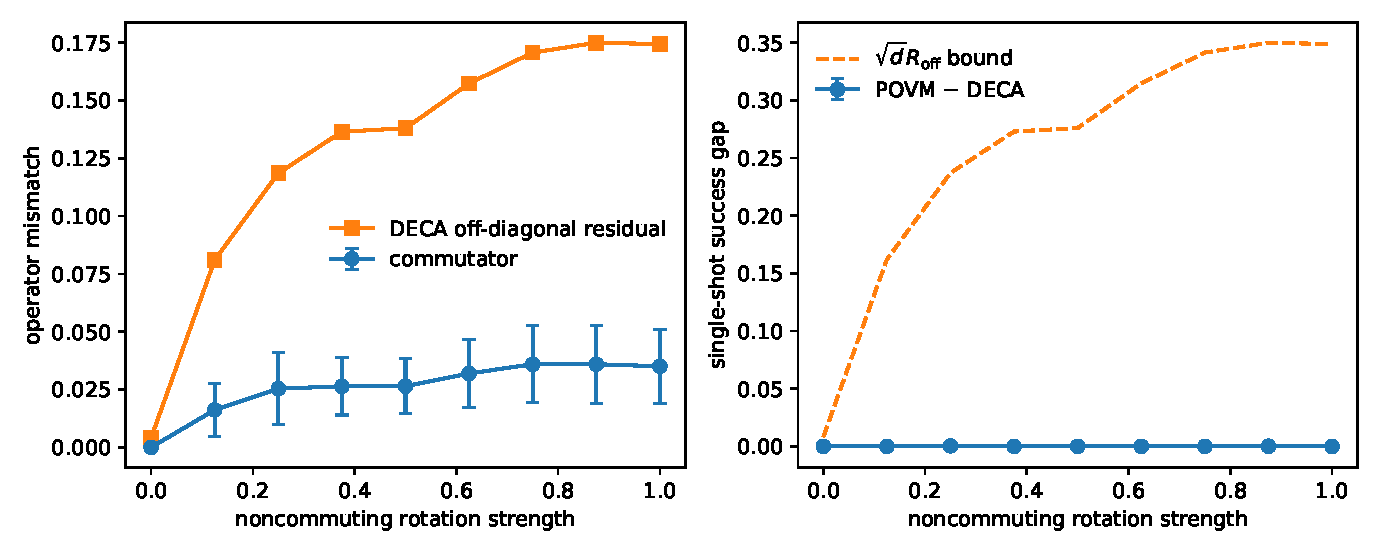
\includegraphics[width=\columnwidth]{noncommutativity_gap.pdf}
\caption{Controlled noncommuting ensembles.  The off-diagonal bound is valid
but loose; rotation strength and commutator norm do not imply a monotone
oracle gap.  Error bars show variation across eight seeds.}
\label{fig:noncommuting}
\end{figure}

\subsection{Circuit validation and POVM advantage}

The maximum total-variation error between Qiskit shot frequencies and analytic
probabilities was $0.0073$.  Binary PVM-DECA achieved analytic training
single-shot success $0.9434$ with no outcome ancilla.  On the equal-prior
trine ensemble, the best commuting PVM found by Jacobi-DECA achieved
$0.6220$, while PGM and the SDP POVM achieved $2/3$, an absolute advantage
$0.04466$.  The general realization used two padded outcome qubits.
\Cref{fig:quantum} reports analytic and sampled success.

\begin{figure}[t]
\centering
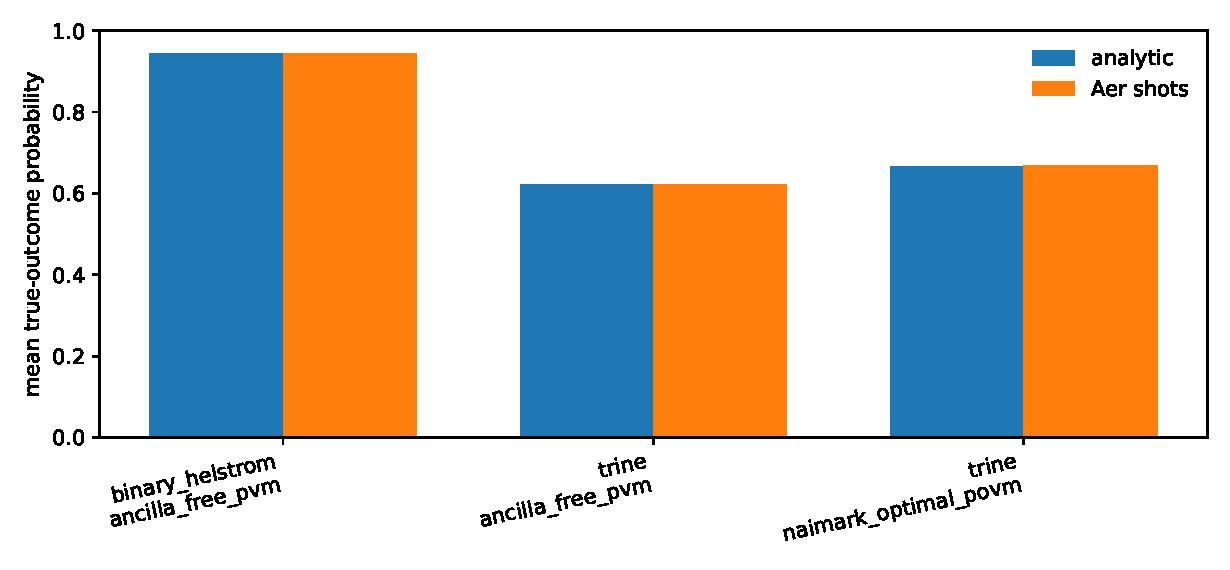
\includegraphics[width=\columnwidth]{quantum_simulation_success.pdf}
\caption{Analytical and 16,384-shot Qiskit Aer success.  The trine ensemble
exhibits a real POVM advantage; the binary PVM is ancilla-free and exact.}
\label{fig:quantum}
\end{figure}

\subsection{Classical mechanism and predictive accuracy}

\Cref{tab:main_accuracy} reports repeated-CV accuracy.  The covariance-only
task demonstrates the intended mechanism: logistic regression is at
$0.496\pm0.019$, whereas Spectral-DECA-amplitude reaches
$0.786\pm0.014$ (shown in the complete table in
\cref{tab:full_accuracy}).  PVM-DECA reaches only $0.623\pm0.038$ because
sign-only Helstrom weights solve a different single-shot objective.  On the
mean-only task, amplitude variants are near chance, while the affine spectral
rule reaches $0.825\pm0.017$, matching logistic regression.

\begin{table*}[t]
\centering
\caption{Accuracy (mean $\pm$ standard deviation over two repeats of
five-fold stratified CV).  A: amplitude encoding; F: affine encoding.
Configurations are fixed rather than nested-tuned.}
\label{tab:main_accuracy}
\resizebox{\textwidth}{!}{\begin{tabular}{lcccccc}
\toprule
Dataset & Logistic & QDA & RBF-SVM & RF & PVM-A & PGM-F \\
\midrule
Covariance signal & 0.496 $\pm$ 0.019 & 0.823 $\pm$ 0.022 & 0.759 $\pm$ 0.017 & 0.824 $\pm$ 0.020 & 0.623 $\pm$ 0.038 & 0.759 $\pm$ 0.027 \\
Mean signal & 0.825 $\pm$ 0.019 & 0.822 $\pm$ 0.016 & 0.775 $\pm$ 0.019 & 0.828 $\pm$ 0.018 & 0.502 $\pm$ 0.042 & 0.826 $\pm$ 0.016 \\
Iris & 0.957 $\pm$ 0.027 & 0.957 $\pm$ 0.035 & 0.960 $\pm$ 0.034 & 0.943 $\pm$ 0.045 & 0.543 $\pm$ 0.085 & 0.887 $\pm$ 0.050 \\
Wine & 0.980 $\pm$ 0.023 & 0.997 $\pm$ 0.009 & 0.978 $\pm$ 0.022 & 0.980 $\pm$ 0.023 & 0.786 $\pm$ 0.055 & 0.980 $\pm$ 0.030 \\
Breast Cancer & 0.977 $\pm$ 0.014 & 0.965 $\pm$ 0.025 & 0.967 $\pm$ 0.029 & 0.954 $\pm$ 0.026 & 0.675 $\pm$ 0.026 & 0.950 $\pm$ 0.026 \\
Digits & 0.971 $\pm$ 0.007 & 0.979 $\pm$ 0.005 & 0.982 $\pm$ 0.005 & 0.977 $\pm$ 0.008 & 0.890 $\pm$ 0.016 & 0.941 $\pm$ 0.015 \\
Banknote & 0.982 $\pm$ 0.008 & 0.981 $\pm$ 0.008 & 1.000 $\pm$ 0.000 & 0.993 $\pm$ 0.004 & 0.708 $\pm$ 0.026 & 0.956 $\pm$ 0.011 \\
Spambase & 0.926 $\pm$ 0.011 & 0.761 $\pm$ 0.008 & 0.933 $\pm$ 0.009 & 0.954 $\pm$ 0.005 & 0.866 $\pm$ 0.008 & 0.854 $\pm$ 0.011 \\
Dry Bean & 0.925 $\pm$ 0.006 & 0.920 $\pm$ 0.005 & 0.931 $\pm$ 0.004 & 0.925 $\pm$ 0.004 & 0.616 $\pm$ 0.004 & 0.829 $\pm$ 0.005 \\
Letter & 0.773 $\pm$ 0.005 & 0.849 $\pm$ 0.004 & 0.971 $\pm$ 0.002 & 0.966 $\pm$ 0.003 & 0.311 $\pm$ 0.010 & 0.617 $\pm$ 0.003 \\
\bottomrule
\end{tabular}
}
\end{table*}

The public-data conclusion is deliberately conservative.  PGM is competitive
on Wine ($0.980$) and trails strong baselines moderately on Breast Cancer
($0.950$) and Digits ($0.941$), but PVM and spectral variants are generally
weaker.  Across the eight public datasets, the Friedman statistic is $57.44$
with $p=1.10\times10^{-8}$.  Dataset-level exploratory Wilcoxon tests with
Holm correction give:
\begin{itemize}
  \item PGM minus PVM: mean $+0.202$, seven wins in eight datasets,
  adjusted $p=0.0469$;
  \item PGM minus RBF-SVM: mean $-0.0886$, one win in eight,
  adjusted $p=0.0469$.
\end{itemize}
Only eight independent dataset blocks are available, so these pairwise tests
are supporting evidence rather than definitive population-level rankings.

Letter Recognition supplies a sharp structural stress test:
$K=26>d=17$ after affine lifting.  In agreement with
\cref{prop:capacity}, PVM-DECA achieves $0.311\pm0.010$; a 26-effect PGM
improves to $0.617\pm0.003$; RBF-SVM reaches $0.971\pm0.002$.
Dry Bean, where $K<d$ but the shared-basis assumption remains restrictive,
similarly separates PVM ($0.616$), PGM ($0.829$), and RBF-SVM ($0.931$).

\begin{figure*}[t]
\centering
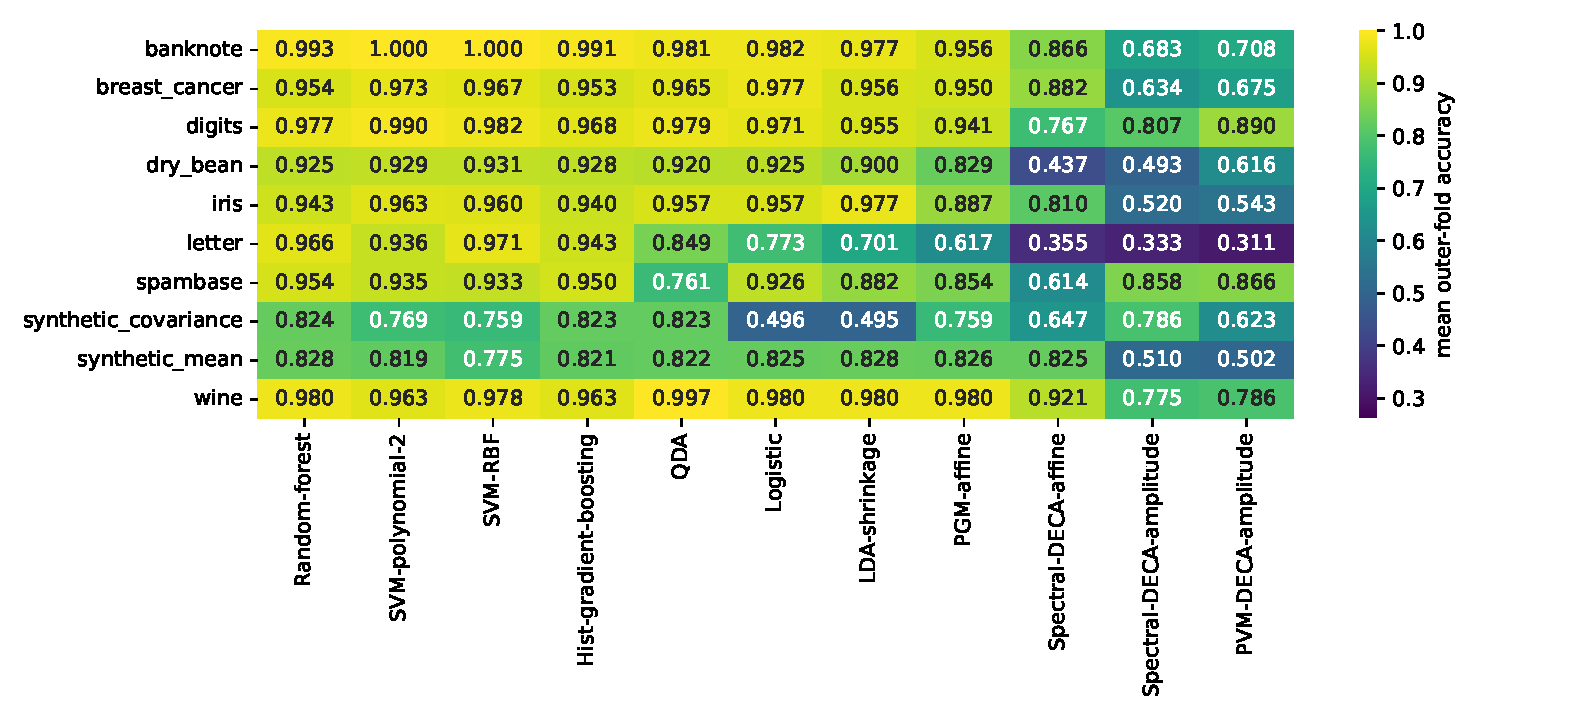
\includegraphics[width=0.98\textwidth]{benchmark_accuracy.pdf}
\caption{Complete mean-accuracy matrix.  The controlled datasets explain
\emph{when} energy contrast works; the public datasets expose the substantial
cost of a shared measurement basis.}
\label{fig:heatmap}
\end{figure*}

\subsection{Resource observations}

\Cref{tab:resources} shows median wall-clock measurements.  Binary DECA fits
are analytical and often millisecond-scale.  Multiclass Jacobi cost grows
with dimension and sweep budget: on Digits, PVM training takes
\SI{2.12}{s}, versus \SI{0.034}{s} for the fixed RBF-SVM configuration and
\SI{0.15}{s} for PGM.  On large, low-dimensional Letter, PVM and PGM prediction
are faster per sample than RBF-SVM but sacrifice large amounts of accuracy.
These software timings are not hardware, power, or asymptotic quantum
advantage measurements.

\begin{table}[t]
\centering
\caption{Median outer-fold software resource measurements.}
\label{tab:resources}
\resizebox{\columnwidth}{!}{\begin{tabular}{llrrr}
\toprule
Dataset & Method & Accuracy & Fit (s) & Predict ($\mu$s/sample) \\
\midrule
Digits & RBF-SVM & 0.982 & 0.03433 & 34.16 \\
 & PVM-A & 0.890 & 2.123 & 77.92 \\
 & PGM-F & 0.941 & 0.15 & 80.38 \\
\addlinespace
Spambase & RBF-SVM & 0.933 & 0.1485 & 32.08 \\
 & PVM-A & 0.866 & 0.06704 & 16.87 \\
 & PGM-F & 0.854 & 0.06983 & 14.92 \\
\addlinespace
Dry Bean & RBF-SVM & 0.931 & 0.214 & 52.96 \\
 & PVM-A & 0.616 & 0.1709 & 4.094 \\
 & PGM-F & 0.829 & 0.06104 & 4.718 \\
\addlinespace
Letter & RBF-SVM & 0.971 & 0.9645 & 221.4 \\
 & PVM-A & 0.311 & 0.4181 & 14.06 \\
 & PGM-F & 0.617 & 0.3396 & 17.84 \\
\bottomrule
\end{tabular}
}
\end{table}

\section{Applications and Design Guidance}
\label{sec:applications}

\paragraph{Native quantum data.}
The strongest use case is measurement design when inputs already are quantum
states: qubit readout, communication receivers, sensing, calibration, and
drift monitoring.  There is no classical state-loading cost.  Binary and
commuting ensembles admit exact ancilla-free measurements; the residual and
SDP gap quantify when a more expensive POVM is justified.

\paragraph{Classical second-order signals.}
Spectral-DECA is most plausible for zero-mean or covariance-dominated
measurements: EEG/BCI, radar and RF, vibration faults, texture or scattering
features, and few-shot normalized embeddings.  The covariance-only experiment
supports this mechanism.  A practitioner should compare class-operator
commutators, fit a common basis, and inspect $R_{\mathrm{off}}$ before assuming
that the shared-basis bias is appropriate.

\paragraph{Decision guide.}
Use binary closed-form DECA when a single physical measurement is the true
loss.  Use Spectral-DECA when eigenvalue magnitude is meaningful and repeated
expectation estimation is available.  Use PGM when multiclass accuracy
justifies nonprojective effects and a closed form is preferred.  Use the SDP
oracle for small validation problems.  If $K>d$, enlarge the encoding, use a
general POVM/Naimark dilation, or use hierarchical measurements.  For ordinary
tabular prediction, strong classical baselines remain mandatory.

\section{Limitations and Reproducibility}
\label{sec:limitations}

First, $\rho_c$ retains only the class average of encoded rank-one operators.
Higher-order and multimodal within-class information can be lost.  Second,
amplitude normalization discards norm; affine lifting introduces a scale that
was fixed rather than nested-tuned here.  Third, the Jacobi objective is
nonconvex.  Monotonicity guarantees objective convergence, not global
optimality or test-accuracy improvement.  Fourth, the bound in
\cref{eq:gap_bound} can be loose and does not reverse: a small actual gap does
not imply a small residual.  Fifth, repeated-CV standard deviations are
descriptive because folds overlap; the independent-block tests use only eight
public datasets.  Sixth, arbitrary state preparation and dense unitaries can
dominate a classical-to-quantum pipeline.  We make no end-to-end speedup claim.

The code records all seeds, versions, URLs, archive hashes, fold predictions,
measurement diagnostics, and generated figures.  Qiskit simulations are local
and require no cloud account.  Authorship and venue metadata in this draft are
placeholders and must be confirmed before submission.

\section{Conclusion}
\label{sec:conclusion}

DECA gives a precise answer to the original ``class difference rather than
variance'' intuition.  The right mathematical object is the spectrum of
class-conditional energy operators, and the right physical interpretation is
an optimal measurement only after its constraints are stated.  A shared
unitary is useless before an unrestricted POVM, but valuable as a compressed,
interpretable measurement basis.  Binary and commuting cases are exact;
noncommuting multiclass cases have a computable residual bound and a monotone
Jacobi approximation.  Retaining eigenvalue magnitudes yields a distinct
spectral quadratic classifier.

The experiments support the theory more strongly than a universal performance
story: DECA succeeds on controlled second-order structure, general POVMs
consistently repair part of the multiclass loss, and ordinary kernel or
ensemble methods remain stronger on most tabular tasks.  This honest boundary
turns ECA from a broad quantum analogy into a falsifiable framework for
discriminative components, measurement compression, and resource-aware
classification.

\appendix

\section{Additional Derivations}

\subsection{Binary basis objective}
For scalars $u,v$, $\max(u,v)=(u+v+|u-v|)/2$.  Therefore
\[
\begin{aligned}
\sum_j\max(p_j^\dagger A_1p_j,p_j^\dagger A_2p_j)
&=\frac12\sum_j p_j^\dagger(A_1+A_2)p_j\\
&\quad+\frac12\sum_j|p_j^\dagger\Delta p_j|\\
&=\frac12\left[1+
\|\diag(P^\dagger\Delta P)\|_1\right].
\end{aligned}
\]
This yields \cref{eq:binary_basis_objective}.

\subsection{Spectral score as a structured quadratic model}
For real affine encoding before its normalization, let
$\widetilde x=[x^\top,\tau]^\top$.  If
$\Delta=P\diag(\lambda)P^\top$, then
\[
\widetilde x^\top\Delta\widetilde x
=\sum_j\lambda_j(p_j^\top\widetilde x)^2.
\]
Partitioning $\Delta$ as
$\left[\begin{smallmatrix}Q&q\\q^\top&q_0\end{smallmatrix}\right]$
gives $x^\top Qx+2\tau q^\top x+\tau^2q_0$.  Spectral-DECA is therefore
linear in learned energy features but quadratic, with possible linear and
bias terms, in the original input.

\section{Complete Accuracy Table}
\label{app:complete}

\begin{table*}[t]
\centering
\caption{Mean accuracy for all methods.  Spec-A and Spec-F denote spectral
DECA with amplitude and affine encodings.  HGB denotes histogram gradient
boosting.}
\label{tab:full_accuracy}
\scriptsize
\resizebox{\textwidth}{!}{\begin{tabular}{lccccccccccc}
\toprule
Dataset & Logistic & LDA & QDA & Poly-SVM & RBF-SVM & RF & HGB & PVM-A & Spec-A & Spec-F & PGM-F \\
\midrule
Covariance signal & 0.496 & 0.495 & 0.823 & 0.769 & 0.759 & 0.824 & 0.823 & 0.623 & 0.786 & 0.647 & 0.759 \\
Mean signal & 0.825 & 0.828 & 0.822 & 0.819 & 0.775 & 0.828 & 0.821 & 0.502 & 0.510 & 0.825 & 0.826 \\
Iris & 0.957 & 0.977 & 0.957 & 0.963 & 0.960 & 0.943 & 0.940 & 0.543 & 0.520 & 0.810 & 0.887 \\
Wine & 0.980 & 0.980 & 0.997 & 0.963 & 0.978 & 0.980 & 0.963 & 0.786 & 0.775 & 0.921 & 0.980 \\
Breast Cancer & 0.977 & 0.956 & 0.965 & 0.973 & 0.967 & 0.954 & 0.953 & 0.675 & 0.634 & 0.882 & 0.950 \\
Digits & 0.971 & 0.955 & 0.979 & 0.990 & 0.982 & 0.977 & 0.968 & 0.890 & 0.807 & 0.767 & 0.941 \\
Banknote & 0.982 & 0.977 & 0.981 & 1.000 & 1.000 & 0.993 & 0.991 & 0.708 & 0.683 & 0.866 & 0.956 \\
Spambase & 0.926 & 0.882 & 0.761 & 0.935 & 0.933 & 0.954 & 0.950 & 0.866 & 0.858 & 0.614 & 0.854 \\
Dry Bean & 0.925 & 0.900 & 0.920 & 0.929 & 0.931 & 0.925 & 0.928 & 0.616 & 0.493 & 0.437 & 0.829 \\
Letter & 0.773 & 0.701 & 0.849 & 0.936 & 0.971 & 0.966 & 0.943 & 0.311 & 0.333 & 0.355 & 0.617 \\
\bottomrule
\end{tabular}
}
\end{table*}

\section{Repository Commands}

{\footnotesize
\begin{verbatim}
python -m pytest experiments/run1/tests -q
cd experiments
python scripts/run_theory_validation.py
python scripts/run_quantum_simulation.py
python scripts/run_classical_benchmarks.py \
  --folds 5 --repeats 2
python scripts/analyze_classical_results.py
python scripts/export_paper_tables.py
cd ..
make -C publication
\end{verbatim}
}

\bibliographystyle{unsrtnat}
\bibliography{references}

\end{document}
